\section{Light Odd-Z Isotope Production}\label{sec:lightoddZ}

The $p$-nuclei are not the sole unique nucleosynthetic feature of O-C shell mergers.
The light odd-Z elements P, Cl, K, and Sc have all been noted as products as well  \cite{ritterConvectivereactiveNucleosynthesisSc2018, robertiOccurrenceImpactCarbonOxygen2025}.
These elements are of interest because they are underproduced in galactic chemical evolution calculations \citep{ritterConvectivereactiveNucleosynthesisSc2018}, there are observations of P-enhanced stars \citep{masseronPhosphorusrichStarsUnusual2020, braunerUnveilingChemicalFingerprint2023, braunerUnveilingChemicalFingerprint2024}, and $\mathrm{K}$ in particular is relevant for the habitability of exoplanets \cite{frankRadiogenicHeatingEvolution2014, oneillEffectGalacticChemical2020}.

Using the same models described in Chapter \ref{chapter:impact_of_3D_nuclear_pnuclei_OCmerger}, I present the preliminary results of how the light odd-Z elements are produced in O-C shell mergers.

\begin{figure}[htbp]
    \centering
    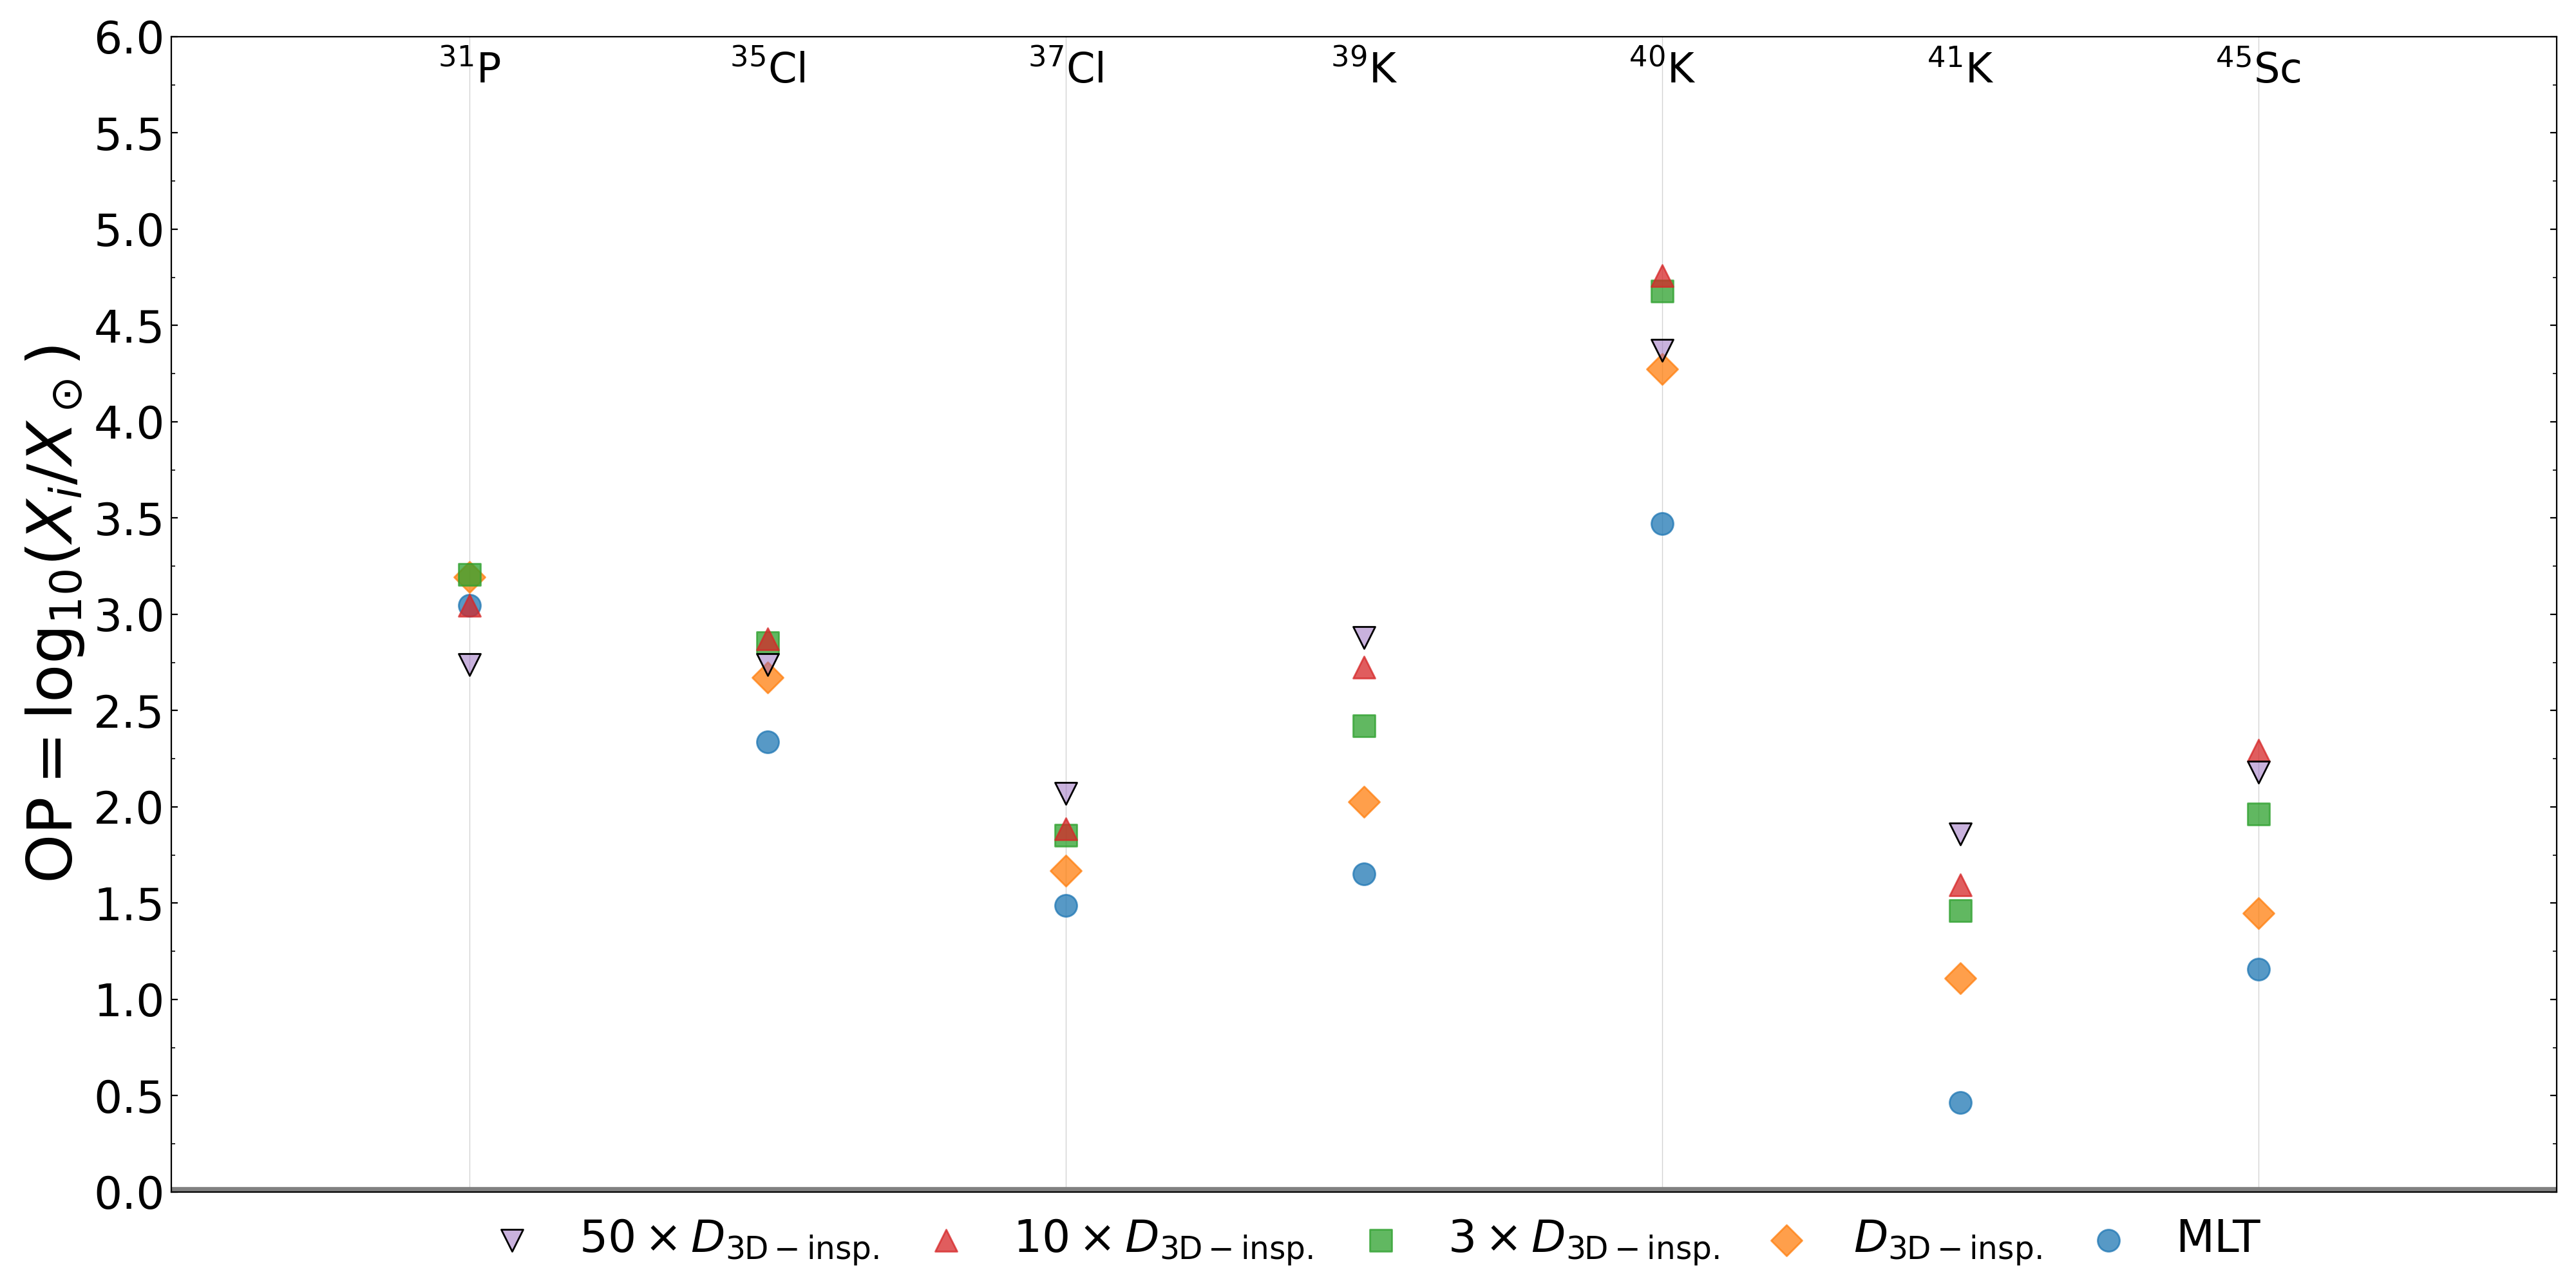
\includegraphics[width=\textwidth]{chapters/3/figures/lightoddz_downturn.png}
    \caption{Impact on the production of the light odd-Z stable isotopes of P, Cl, K, and Sc comparing MLT and convective dowturn models.}
    \label{fig:lightoddZ_production}
\end{figure}

As Figure \ref{fig:lightoddZ_production} shows, the light odd-Z elements are all clearly effected by the presence of a convective downturn. 
Similar to the $p$-nuclei, the impact is non-monotonic and non-linear, as $^{31}\mathrm{P}$, $^{35}\mathrm{Cl}$, $^{40}\mathrm{K}$, and $^{45}\mathrm{Sc}$ all decrease in production at the fastest mixing speeds.
K and Sc show the most significant impact from the convective downturn with a spread in production of $1.5-2$ orders of magnitude.

\jitxt{I have more plots and tables I can add here if we want to do that}
\begin{itemize}
    \item Tables for each mixing case showing the relevant reactions that each species undergoes
    \item Plots showing how the convective profiles change the mass fraction profiles of K-39, K-40, K-41 including GOSH and partial merger (with cool dips)
    \item I can make the impact on production with GOSH and partial merger too
    \item I have plots showing the impact from ingestion
    \item XRISM collaboration Ne/O vs K/Ar plots that show a clear trend for both the mixing speeds and ingestion rate
\end{itemize}